\paragraph{\texttt{ArticleCard}}  \mbox{}\\

This component displays a card for a given article, including its title, a brief excerpt of its content,
and the date of publication. Prior to \texttt{CourseCard}, the first table of is relatively straightforward.


\begin{center}
    \begin{tabularx}{\textwidth}{|X|X|X|X|}
        \hline
        \textbf{Prop} & Type & Required & Description \\
        \hline
        \texttt{article} & \texttt{Article} & yes & A yoga article \\
        \hline
    \end{tabularx}
\end{center}

And more precisely

\begin{center}
    \begin{tabularx}{\textwidth}{|X|X|X|}
        \hline
        \textbf{Prop.attribute} & Type & Description \\
        \hline
        \texttt{article.image} & \texttt{string | null} &  the path of the image associated with the yoga article stored in Supabase\\
        \hline
        \texttt{article.title} & \texttt{string} & the title of the yoga article\\
        \hline
        \texttt{article.published\_at} & \texttt{string} & the publication date of the article\\
        \hline
        \texttt{article.content} & \texttt{string} & a snippet of the article's content (maximum 250 characters)\\
        \hline
    \end{tabularx}
\end{center}

\begin{figure}[H]
    \centering
    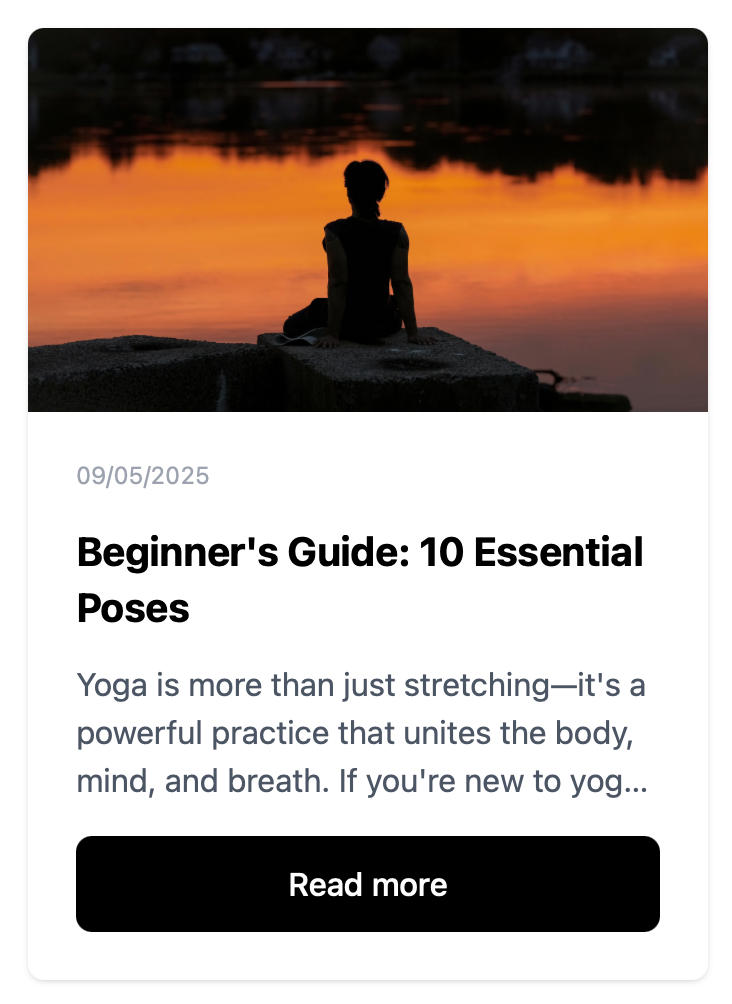
\includegraphics[width=0.2\textwidth]{asset/articleCard}
    \caption{\texttt{ArticleCard}}
\end{figure}